\section{Monday, September 23, 2019}

Today, we'll talk about some more details about returning values from a method, which may have not been mentioned before.

\subsection{Pass By Value}

First, we'll talk about some important details regarding using passed in variables in a method.


Consider the following code segment:

\begin{lstlisting}
public void task(int x) {
    x = x + 1;
}
public static void main(String args[]) {
    int y = 5;
    task(y);
    System.out.println(y);
}
\end{lstlisting}

\begin{enumerate}
    \item In our main method, we initialize a variable \verb!y!, and we set it to the integer $5$. 
    \item Next, we call \verb!task! which simply increments its parameter. 
    \item Finally, we print out the variable $\verb!y!$ in our main method. What value gets printed? 
\end{enumerate}

Possibly surprisingly, the answer is $5$. Why? Because when variables are passed in to a method in Java, the method first makes a copy of all of the variables. The copied variable is what is used inside of the method. In other words, changes to a method's parameters are only local; they are not exhibited when we return back to the main method. \\


This can be confusing --- here's another example:

\begin{lstlisting}
public static void wrongSwap(int a, int b) {
    int temp = a;
    a = b;
    b = temp;
    System.out.println("a: " + a + "b: " + b);
}
public static void main(String args[]) {
    int x = 2, y = 3;
    wrongSwap(x, y);
    System.out.println("x: " + x + "y: " + y);
}
\end{lstlisting}

An unaware programmer might think that, after we call the \verb!wrongSwap! method, the values of \verb!y! and \verb!y! are interchanged. However, as we've discussed, what will actually happen is that we'll make a copy of \verb!x! and \verb!y! to be used in the method. Thus, change takes place (the value of \verb!x! and \verb!y! are still $2$ and $3$, respectively). \\

This construct of making a copy of the variable to be used in the method is known as \vocab{passing by value} (some other programming languages reflect changes made to a parameter in a method; this construct is known as \vocab{passing by reference}). 

\subsection{StringBuffers}

As we've discussed in the past, strings are immutable --- there isn't any way in which we can change the object itself, but we can change the reference to the object. 

The \verb!StringBuffer! class is a peer class of \verb!String!, and it provides many of the functionalities that we'd want to perform on strings. While strings are fixed-length, immutable character sequences, a \verb!StringBuffer! object can be used to represent growable and writable character sequences. More precisely, the \verb!StringBuffer! class is used to create mutable strings. \\

Some of the most commonly used methods on the \verb!StringBuffer! class are listed below:

\begin{itemize}
    \item The \verb!append()! method is used to append a sequence of characters to the end of the current string in the \verb!StringBuffer!.
    \item The \verb!insert()! method is used to insert a sequence of characters into the middle of the current string.
    \item The \verb!length()! method returns the length (character count) of the current string.
\end{itemize}

Here's an example:

\begin{lstlisting}
public static void main(String args[]) {
    int x = 2, y = 3;
    StringBuffer a = new StringBuffer("talk");
    a.append("ing");
    System.out.println(a);
}
\end{lstlisting}

As we'd expect, once we append \verb!ing! to \verb!talk!, we end up printing \verb!talking!. \\


However, it is important to remember that \verb!StringBuffer! have \textit{references} to strings. Thus, if we pass in a \verb!StringBuffer! to a method, and if we modify the \verb!StringBuffer! inside of that method, then we'll end up modifying the string that it points to. Here's another example:


\begin{lstlisting}
public static void addEnding(StringBuffer b) {
    b.append("ing");
    b = null;
}

public static void main(String args[]) {
    StringBuffer a = new StringBuffer("talk");
    addEnding(a);
    System.out.println(a);
}
\end{lstlisting}

As mentioned previously, this code segment will end up printing \verb!talking!. \\
 
Would this work with just a \verb!String! object (not a \verb!StringBuffer!)? No --- recall that \verb!String! objects are immutable; even if we were to append to a string with \verb!+=!, we wouldn't be modifying the original object.


\subsection{Returning Values}

As we have already seen, one of the purposes of returning values in a method is way for us to access the results of a computation performed in the method in our main method. The method call in the \verb!main! is always replaced by what the method returns. 

This is demonstrated below:

\begin{lstlisting}
public int add(int x, int y) {
    return (x + y);
}
public static void main(String args[]) {
    int z = add(5, 4);
    System.out.println(z);
}
\end{lstlisting}

When we execute this code, the \verb!add(5, 4)! call inside of the main method gets replaced with the value that the method returns. In this case, that value is $9$. Thus, the print statement that follows the method call prints out $9$. 
Here's another example of a method:

\begin{lstlisting}
public int maximum(int x, int y) {
    int max;
    if (x >= y) {
        max = x;
    } else {
        max = y;
    }
    return max;
}
\end{lstlisting}

In this method, we take in two integers. We determine which integer is larger than the other, and we return the larger of the two integers. Methods can also have more than one \verb!return! statement. For example, we can rewrite the method above as follows:

\begin{lstlisting}
public int maximum(int x, int y) {
    if (x >= y) {
        return x;
    } else {
        return y;
    }
}
\end{lstlisting}

In this rewritten method, we no longer create the variable \verb!max! to store the maximum value of \verb!x! and \verb!y!. Instead, we just exit the function and the return the maximum value as soon as we know what it is. Once we execute a \verb!return! statement, we no longer execute any of the statements in the method that proceed the \verb!return! statement. \\


We can also use \verb!return! statements to exit early out of \verb!void! methods. Here's an example:

\begin{lstlisting}
public void foo(int x) {
    if (x <= 0) {
        return;
    }
    System.out.println(2*x);
}
\end{lstlisting}

What does this method do? If we pass in a positive number, then we print out the double of that number. Otherwise, we don't do anything. 


\subsection{Software Development}

There are many aspects that come into play when developing software or large-scale programs. We can describe the development of software using \vocab{the software lifecycle}, which is depicted below:


\begin{figure}[h]
    \centering
    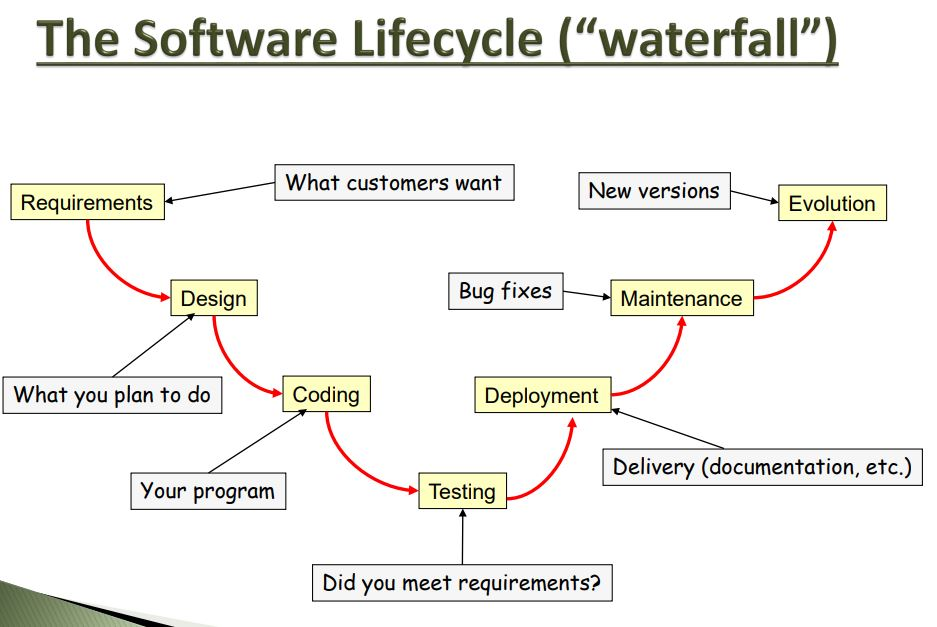
\includegraphics[scale=0.6]{media/lifecycle}
    \caption{Software Development Lifecycle}
    \label{fig:my_label}
\end{figure}

As shown above, software development typically starts by recognizing the requirements the software must satisfy. This consideration typically involves thinking about what customers want. Next, we go into the design phase in which we think about what we plan to do. Finally, we go into the coding phase, followed by testing, deployment, maintenance, and finally evolution. 

When developing software, it's also usually helpful to take a \vocab{top-down approach}. A top-down design is a method of ordering knowledge in which we start from a big idea (i.e. what we want to implement), and we break it down into what we need to achieve what's at the top (and we subsequently break those things down, and so on).


\vocab{Pseudocode} is also useful in creating software. Pseudocode is an English-like description of the set of steps required to solve a problem. Here's an example of some pseudocode for finding the minimum value from numerous inputted numbers.


\begin{center}
\line(1,0){400}
\end{center}

\begin{allintypewriter}

FIND\_MINIMUM \string{

\hspace{0.5cm} read the number of values to process; call this value N.

\hspace{0.5cm} repeat the following steps until N input values have been processed \string{

\hspace{1cm} read the next value into x

\hspace{1cm} if x is the first value read, set the current minimum to x.

\hspace{1cm} otherwise, if x is less than the current minimum, then set the current minimum to x.

\hspace{0.5cm} \string}

\string}

\begin{center}
\line(1,0){400}
\end{center}
\end{allintypewriter}

By using pseudocode, we can avoid having to deal with the subtleties of our programming language's syntax and semantics, and we can instead focus on determining the high-level steps necessary to solve a problem. 